% =====================================================
% ĐƯỜNG TRÒN NGOẠI TIẾP TAM GIÁC ABC
% Hình học phẳng - TikZ LaTeX
% =====================================================

\documentclass[border=5pt,tikz,12pt]{standalone}
\usepackage[utf8]{vietnam}
\usetikzlibrary{calc,intersections}

\begin{document}
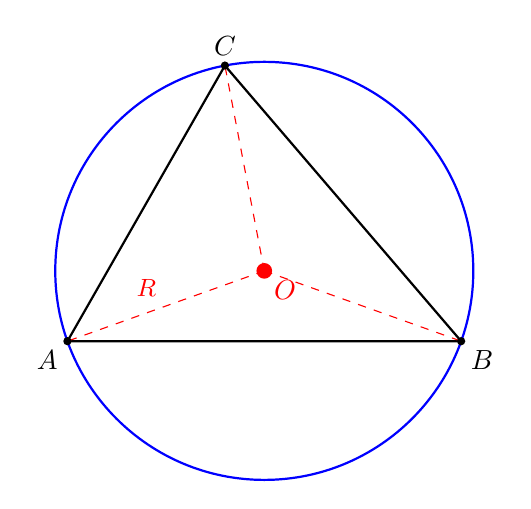
\begin{tikzpicture}[
    % === ĐỊNH NGHĨA STYLE ===
    point/.style={circle, fill, inner sep=1.5pt},
    main line/.style={thick},
    circle line/.style={thick, blue},
    radius line/.style={dashed, red, thin},
    center point/.style={circle, fill=red, inner sep=2pt},
]
    % === ĐỊNH NGHĨA ĐỈNH TAM GIÁC ===
    % Tam giác nhọn để đường tròn ngoại tiếp có tâm nằm trong
    \coordinate (A) at (0,0);
    \coordinate (B) at (5,0);
    \coordinate (C) at (2,3.5);

    % === TÍNH TÂM ĐƯỜNG TRÒN NGOẠI TIẾP ===
    % Tâm O là giao điểm của các đường trung trực
    % Sử dụng công thức tính tâm ngoại tiếp

    % Trung điểm các cạnh
    \coordinate (M_AB) at ($(A)!0.5!(B)$);
    \coordinate (M_BC) at ($(B)!0.5!(C)$);
    \coordinate (M_CA) at ($(C)!0.5!(A)$);

    % Tính tâm O bằng công thức giải tích
    % O là giao của trung trực AB và trung trực BC
    \pgfmathsetmacro{\ax}{0}
    \pgfmathsetmacro{\ay}{0}
    \pgfmathsetmacro{\bx}{5}
    \pgfmathsetmacro{\by}{0}
    \pgfmathsetmacro{\cx}{2}
    \pgfmathsetmacro{\cy}{3.5}

    % Công thức tâm đường tròn ngoại tiếp
    \pgfmathsetmacro{\D}{2*(\ax*(\by-\cy) + \bx*(\cy-\ay) + \cx*(\ay-\by))}
    \pgfmathsetmacro{\Ox}{((\ax*\ax+\ay*\ay)*(\by-\cy) + (\bx*\bx+\by*\by)*(\cy-\ay) + (\cx*\cx+\cy*\cy)*(\ay-\by))/\D}
    \pgfmathsetmacro{\Oy}{((\ax*\ax+\ay*\ay)*(\cx-\bx) + (\bx*\bx+\by*\by)*(\ax-\cx) + (\cx*\cx+\cy*\cy)*(\bx-\ax))/\D}

    \coordinate (O) at (\Ox, \Oy);

    % Bán kính R = khoảng cách từ O đến A
    \pgfmathsetmacro{\R}{sqrt((\Ox-\ax)^2 + (\Oy-\ay)^2)}

    % === VẼ ĐƯỜNG TRÒN NGOẠI TIẾP ===
    \draw[circle line] (O) circle (\R);

    % === VẼ TAM GIÁC ===
    \draw[main line] (A) -- (B) -- (C) -- cycle;

    % === VẼ CÁC BÁN KÍNH (tùy chọn) ===
    \draw[radius line] (O) -- (A);
    \draw[radius line] (O) -- (B);
    \draw[radius line] (O) -- (C);

    % === ĐÁNH DẤU TÂM O ===
    \node[center point] at (O) {};

    % === ĐÁNH DẤU CÁC ĐỈNH ===
    \foreach \p in {A,B,C} \fill (\p) circle (1.5pt);

    % === NHÃN ===
    \node[below left] at (A) {$A$};
    \node[below right] at (B) {$B$};
    \node[above] at (C) {$C$};
    \node[below right, red] at (O) {$O$};

    % === NHÃN BÁN KÍNH (tùy chọn) ===
    \node[red, font=\small] at ($(O)!0.5!(A)$) [above left] {$R$};

\end{tikzpicture}
\end{document}
